% Options for packages loaded elsewhere
\PassOptionsToPackage{unicode}{hyperref}
\PassOptionsToPackage{hyphens}{url}
%
\documentclass[
]{article}
\usepackage{amsmath,amssymb}
\usepackage{iftex}
\ifPDFTeX
  \usepackage[T1]{fontenc}
  \usepackage[utf8]{inputenc}
  \usepackage{textcomp} % provide euro and other symbols
\else % if luatex or xetex
  \usepackage{unicode-math} % this also loads fontspec
  \defaultfontfeatures{Scale=MatchLowercase}
  \defaultfontfeatures[\rmfamily]{Ligatures=TeX,Scale=1}
\fi
\usepackage{lmodern}
\ifPDFTeX\else
  % xetex/luatex font selection
\fi
% Use upquote if available, for straight quotes in verbatim environments
\IfFileExists{upquote.sty}{\usepackage{upquote}}{}
\IfFileExists{microtype.sty}{% use microtype if available
  \usepackage[]{microtype}
  \UseMicrotypeSet[protrusion]{basicmath} % disable protrusion for tt fonts
}{}
\makeatletter
\@ifundefined{KOMAClassName}{% if non-KOMA class
  \IfFileExists{parskip.sty}{%
    \usepackage{parskip}
  }{% else
    \setlength{\parindent}{0pt}
    \setlength{\parskip}{6pt plus 2pt minus 1pt}}
}{% if KOMA class
  \KOMAoptions{parskip=half}}
\makeatother
\usepackage{xcolor}
\usepackage[margin=1in]{geometry}
\usepackage{longtable,booktabs,array}
\usepackage{calc} % for calculating minipage widths
% Correct order of tables after \paragraph or \subparagraph
\usepackage{etoolbox}
\makeatletter
\patchcmd\longtable{\par}{\if@noskipsec\mbox{}\fi\par}{}{}
\makeatother
% Allow footnotes in longtable head/foot
\IfFileExists{footnotehyper.sty}{\usepackage{footnotehyper}}{\usepackage{footnote}}
\makesavenoteenv{longtable}
\usepackage{graphicx}
\makeatletter
\def\maxwidth{\ifdim\Gin@nat@width>\linewidth\linewidth\else\Gin@nat@width\fi}
\def\maxheight{\ifdim\Gin@nat@height>\textheight\textheight\else\Gin@nat@height\fi}
\makeatother
% Scale images if necessary, so that they will not overflow the page
% margins by default, and it is still possible to overwrite the defaults
% using explicit options in \includegraphics[width, height, ...]{}
\setkeys{Gin}{width=\maxwidth,height=\maxheight,keepaspectratio}
% Set default figure placement to htbp
\makeatletter
\def\fps@figure{htbp}
\makeatother
\setlength{\emergencystretch}{3em} % prevent overfull lines
\providecommand{\tightlist}{%
  \setlength{\itemsep}{0pt}\setlength{\parskip}{0pt}}
\setcounter{secnumdepth}{5}
\newlength{\cslhangindent}
\setlength{\cslhangindent}{1.5em}
\newlength{\csllabelwidth}
\setlength{\csllabelwidth}{3em}
\newlength{\cslentryspacingunit} % times entry-spacing
\setlength{\cslentryspacingunit}{\parskip}
\newenvironment{CSLReferences}[2] % #1 hanging-ident, #2 entry spacing
 {% don't indent paragraphs
  \setlength{\parindent}{0pt}
  % turn on hanging indent if param 1 is 1
  \ifodd #1
  \let\oldpar\par
  \def\par{\hangindent=\cslhangindent\oldpar}
  \fi
  % set entry spacing
  \setlength{\parskip}{#2\cslentryspacingunit}
 }%
 {}
\usepackage{calc}
\newcommand{\CSLBlock}[1]{#1\hfill\break}
\newcommand{\CSLLeftMargin}[1]{\parbox[t]{\csllabelwidth}{#1}}
\newcommand{\CSLRightInline}[1]{\parbox[t]{\linewidth - \csllabelwidth}{#1}\break}
\newcommand{\CSLIndent}[1]{\hspace{\cslhangindent}#1}
\usepackage{booktabs}
\usepackage{longtable}
\usepackage{array}
\usepackage{multirow}
\usepackage{wrapfig}
\usepackage{float}
\usepackage{colortbl}
\usepackage{pdflscape}
\usepackage{tabu}
\usepackage{threeparttable}
\usepackage{threeparttablex}
\usepackage[normalem]{ulem}
\usepackage{makecell}
\usepackage{xcolor}
\ifLuaTeX
  \usepackage{selnolig}  % disable illegal ligatures
\fi
\IfFileExists{bookmark.sty}{\usepackage{bookmark}}{\usepackage{hyperref}}
\IfFileExists{xurl.sty}{\usepackage{xurl}}{} % add URL line breaks if available
\urlstyle{same}
\hypersetup{
  pdftitle={NHANES Blood Pressure-Based Mortality Risk - Appendix},
  pdfauthor={Rscripts by Hamish Patten, DW Bester and David Steinsaltz},
  hidelinks,
  pdfcreator={LaTeX via pandoc}}

\title{NHANES Blood Pressure-Based Mortality Risk - Appendix}
\author{Rscripts by Hamish Patten, DW Bester and David Steinsaltz}
\date{10/10/2023}

\begin{document}
\maketitle

{
\setcounter{tocdepth}{3}
\tableofcontents
}
\hypertarget{appendix-a-the-data}{%
\section{Appendix A -- The data}\label{appendix-a-the-data}}

\begin{figure}

{\centering 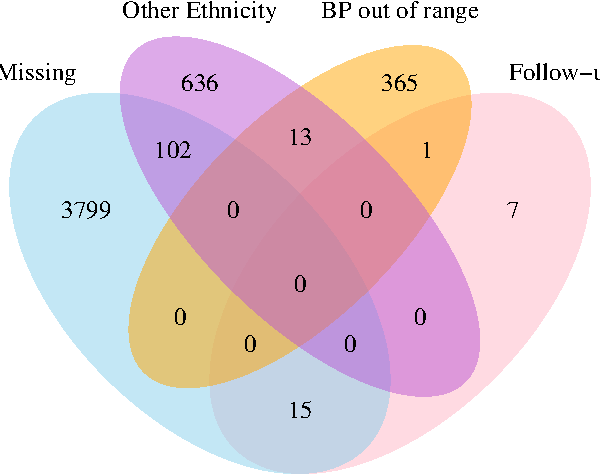
\includegraphics{fig_test_files/figure-latex/Venn1-1} 

}

\caption{Venn diagram of subjects excluded from the analysis.}\label{fig:Venn1}
\end{figure}

\hypertarget{exclusions}{%
\subsection{Exclusions}\label{exclusions}}

There were 19592 subjects in the initial data set.
Of these 4573 were excluded because they had missing data or were not followed up, or belonged to the ``Other'' ethnic group.
This left 15019 subjects for further consideration.
A small number of subjects were excluded because their blood pressure measurements were outside the normal range, as described below in section \ref{sec:BPrange}.
In the end there were 14654 subjects in the analysis data set.
A Venn diagram of the different causes of exclusion is given in Figure \ref{fig:Venn1}.
We will refer to this as the ``full population''.
Of these, 9008 had a computable FRS score.
We call this the ``FRS population''.

\hypertarget{addressing-errors-in-blood-pressure-measurement}{%
\subsection{Addressing errors in blood pressure measurement}\label{addressing-errors-in-blood-pressure-measurement}}

The blood pressure measurement or recording errors were found particularly in the home measurements.
While these did not destroy the usefulness of the home measurements, they did require some attention and decisions for how to work with these defects.
We also consider them inherently interesting, and worth registering for future researchers working on these or similar data.
In particular, the problem we have called ``dependent replication'' was entirely unexpected, although not unprecedented, and is of particular concern to researchers trying to estimate individual variation in clinically relevant measures.

\hypertarget{sec:lastdigit}{%
\subsubsection{Last-digit preference}\label{sec:lastdigit}}

Mild tendency for observers to prefer certain last digits in reporting BP measurements has been reported in other studies, though an analysis of the 1999 wave of NHANES reported no last-digit preference (Ostchega et al. 2003).\\
The last-digit preference in NHANES III, on the other hand, is substantial, with about 26.7\% of all the clinic-measured systolic BP measurements ending in 0, but only about 31.9\% ending in 4 or 6. Because the shifts due to last-digit preference are presumably small, we expect them to have little effect on the main effects that we are examining in this paper, but they do increase the probability of two measurements being rounded to the same value, something that needs to be taken into account in examining the problem of dependent replication.

\begin{table}[!h]

\caption{\label{tab:digit-summary}Summary data for BP end digits}
\centering
\begin{tabular}[t]{llrrrrr}
\toprule
Place & Sys/Dias & 0 & 2 & 4 & 6 & 8\\
\midrule
Home & Systolic & 0.240 & 0.199 & 0.159 & 0.169 & 0.233\\
Home & Diastolic & 0.186 & 0.179 & 0.198 & 0.217 & 0.219\\
Clinic & Systolic & 0.267 & 0.188 & 0.160 & 0.159 & 0.226\\
Clinic & Diastolic & 0.192 & 0.189 & 0.209 & 0.212 & 0.198\\
\bottomrule
\end{tabular}
\end{table}

\hypertarget{sec:pseudorep}{%
\subsubsection{Dependent replicates}\label{sec:pseudorep}}

While the protocol calls for each subject to have three independent BP measures taken, it is not impossible that the observers may have been influenced by one measure in recording the next.
This could happen in either direction: later measurements could be pulled closer to the first, or there could be an inclination to avoid repeated measures.
This is relevant, because erroneously repeated measures would artificially decrease the variance of the three measurements, and avoiding repeated measures would have the opposite effect.

The end-digit bias may be expected to have an effect here, since it influences the probability of two measurements being rounded to the same value.
We begin by noting the standard deviations for measurements of individual subjects as given in the column `Mean of SD' in Table \ref{tab:sd-summary}.
The column `Prob all rep' gives the theoretical probability that two of the three measurements for a subject would have the same value, if the measurements were independent and normally distributed with the given standard deviation (adjusted for the rounding), and assuming that rounding to particular digits is done in proportion to the fractions listed in Table \ref{tab:digit-summary}.
The column `Prob 2 rep' gives the probability that two of the three measurements would have the same value, under the same conditions.
The column `Frac all rep' gives the observed fraction of subjects for whom all three measurements were equal, and `Frac 2 rep' gives the fraction for whom two of the three measurements were equal.
The observed fractions for three equal measurements are all very close to the theoretical probabilities, but the observed fractions for two equal measurements are substantially lower than the theoretical probabilities.
(For comparison, a 95\% probability range for the fraction of subjects with two equal measurements is about \(\pm 0.008\).)

In Figure \ref{fig:examinerPlot}, we show the fraction of subjects with two equal measurements, by examiner, blocked by place and type.
We see that the fraction of subjects with two equal measurements varies substantially by examiner, and that the variation is greater for the systolic than for the diastolic measurements.

\begin{table}[!h]

\caption{\label{tab:sd-summary}Summary data for repeated measures}
\centering
\begin{tabular}[t]{llrrrrr}
\toprule
Place & Sys/Dias & Mean of SD & Frac all rep & Prob all rep & Frac 2 rep & Prob 2 rep\\
\midrule
Home & Systolic & 2.739 & 0.050 & 0.048 & 0.432 & 0.510\\
Home & Diastolic & 2.343 & 0.063 & 0.061 & 0.488 & 0.564\\
Clinic & Systolic & 3.775 & 0.024 & 0.028 & 0.355 & 0.400\\
Clinic & Diastolic & 3.082 & 0.028 & 0.036 & 0.414 & 0.459\\
\bottomrule
\end{tabular}
\end{table}

\begin{figure}
\centering
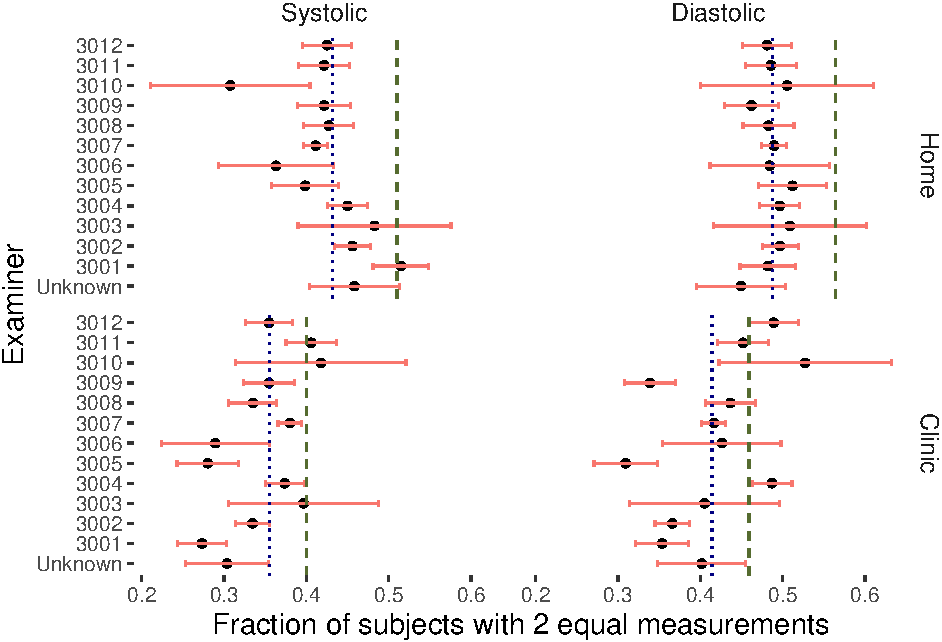
\includegraphics{fig_test_files/figure-latex/examinerPlot-1.pdf}
\caption{\label{fig:examinerPlot}Number of subjects with 2 equal measurements by examiner, blocked by place and type. Red band shows 95\% probability range. Vertical green dashed line shows expected fraction; blue dotted line shows observed fraction over all examiners.}
\end{figure}

\begin{figure}
\centering
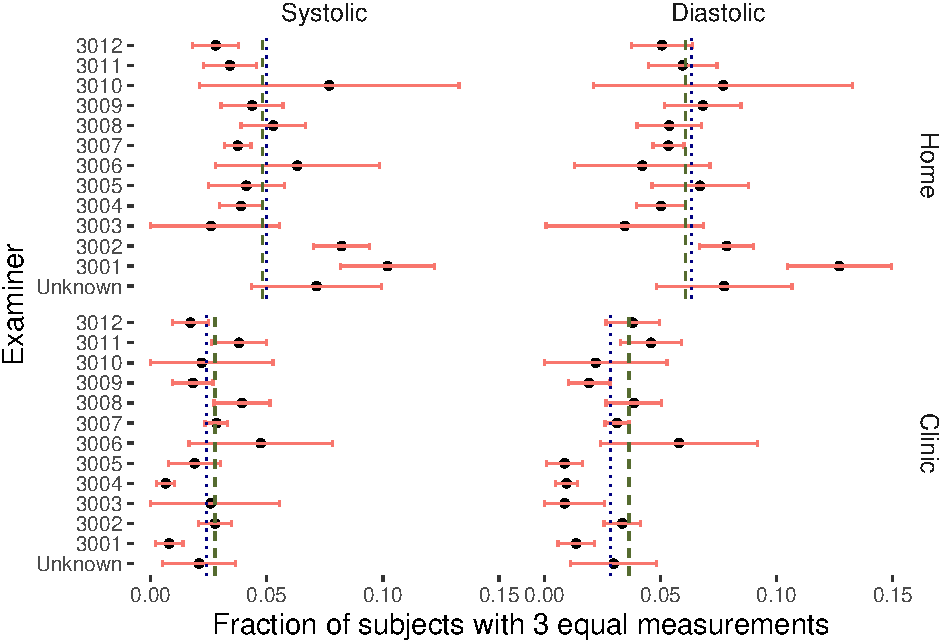
\includegraphics{fig_test_files/figure-latex/examinerPlot3-1.pdf}
\caption{\label{fig:examinerPlot3}Number of subjects with 3 equal measurements by examiner, blocked by place and type. Red band shows 95\% probability range. Vertical green dashed line shows expected fraction; blue dotted line shows observed fraction over all examiners.}
\end{figure}

In Figure \ref{fig:examinerPlot3}, we show the fraction of subjects with three equal measurements, by examiner, blocked by place and type.
Relative to the expected random fluctuations, we see that there is even more variation among the examiners.
One examiner (3001) produced consistently excessive numbers of triple repeats in Home measurements, and a deficit of triple repeats in Clinic measurements.

One further point to explore is the position of the two equal measures in a group of three.
If there are three independent measures, with two equal, each of the three has equal probability of being the odd one out.
On the other hand, if there is a trend in the measurements, then the second is least likely to be the odd one out.

In fact, what we observe is that it is the third measurement that is least likely to differ from the other two, while the first is most likely.
This is what we would expect if examiners sometimes either intentionally copied the second measurement into the space for the third, or unintentionally allowed themselves to be influenced into observing the same number.
The proportions are listed in Table \ref{tab:ternary}.
A chi-squared test for difference from the expected equal proportions for each site and type is shown in Table \ref{tab:proportionChisq}.

We see that there is a huge deviation from the expected proportions in the Home measurements, but less in the Home measurements, and more deviation in Systolic than in Diastolic measurements.

\begin{table}[!h]

\caption{\label{tab:proportionChisq}Chi-square test for difference between observed proportions (all examiners), stratified by place and type}
\centering
\begin{tabular}[t]{llrrrrl}
\toprule
Place & Sys/Dias & Freq1 & Freq2 & Freq3 & ChiSq & p-value\\
\midrule
Home & Systolic & 2657 & 2149 & 1522 & 306.0 & 3.57e-67\\
Home & Diastolic & 2864 & 2541 & 1746 & 278.0 & 4.3e-61\\
Clinic & Systolic & 1905 & 1702 & 1594 & 28.8 & 5.57e-07\\
Clinic & Diastolic & 2172 & 1992 & 1906 & 18.2 & 1.12e-04\\
\bottomrule
\end{tabular}
\end{table}

To explore this further, we can look at the proportions of first, second and third measurements from each examiner that are different from the other two.
The results of a chi-squared test for each examiner (stratified by site and type of BP) for difference from the expected equal proportions are shown in Figure \ref{fig:proportionChisq2}.
The dashed line represents a p-value of 0.001.
Here we see that the Home measurements are extremely variable, while the Clinic measurements are quite consistent with the expected proportions, with the single exception of examiner 3004, who is far from the expected equal proportions in all categories of measurement.

\hypertarget{refs}{}
\begin{CSLReferences}{1}{0}
\leavevmode\vadjust pre{\hypertarget{ref-ostchega2003national}{}}%
Ostchega, Yechiam, Ronald J Prineas, Ryne Paulose-Ram, Carlene M Grim, Grace Willard, and Doreen Collins. 2003. {``National Health and Nutrition Examination Survey 1999-2000: Effect of Observer Training and Protocol Standardization on Reducing Blood Pressure Measurement Error.''} \emph{Journal of Clinical Epidemiology} 56 (8): 768--74.

\end{CSLReferences}

\end{document}
